% ==================================================
% Appendix: Uncertainty in cluster positions %
% ==================================================

%TODO : Organize figure positioning once you're done writing. 

\chapter[Cluster position uncertainty]{Uncertainty in cluster positions}
\label{appendix:clustering}

% Cluster def
% Cluster x from wires, cluster y from strips
% Cluster x uncertainty -- not needed in this
% Cluster y statistical uncertainty
% Cluster y systematic uncertainty depending on choice of fitting algorithm

% --------------------------------------------------
% \section{Cluster definition}
% --------------------------------------------------
%\label{sec:appendix_clustering_cluster_def}

%A cluster is a series of contiguous strip channels on a layer with non-zero amplitude, all part of the same trigger and having the same event number~\cite{lefebvre_thesis}. Clusters result from the drift of ionization products generate in the ionization avalanche caused by a muon~\cite{townsend_electricity_1915}. The peak-detector-output (PDO) of the signal on each strip of a cluster is fit with a Gaussian. The y-position of a particle as it passed through the layer is mean of the cluster, referred to here as the hit position.

% --------------------------------------------------
% \section{Effect of fit algorithm on cluster mean}
% --------------------------------------------------
% \label{sec:appendix_clustering_cluster_fit}

Cluster centroids are better modeled by a Gaussian fit than a simple weighted mean because the Gaussian tails better take into account the charge deposited on the outer strips. Also, the Gaussian fit is less biased by differential non-linearity~\cite{lefebvre_thesis}. 

No uncertainty on the peak signal amplitudes of a cluster are assigned since clusters are not built from samples of a Gaussian distribution but instead are digitized measurements of signal amplitude versus position.

The clusters were fit with Guo's method~\cite{guo_simple_2011} and Minuit2 for ROOT~\cite{hatlo_developments_2005}. Guo's method is an analytic solution that takes into account noise, which is good for computational scalability. Minuit2 is the standard fitting algorithm used in particle physics at ATLAS. The difference in cluster means between the two algorithms for all clusters recorded on a given quadruplet is shown in Figure~\ref{fig:mu_reclustering_minus_mu_cosmics}.

\begin{figure}
    \centering
    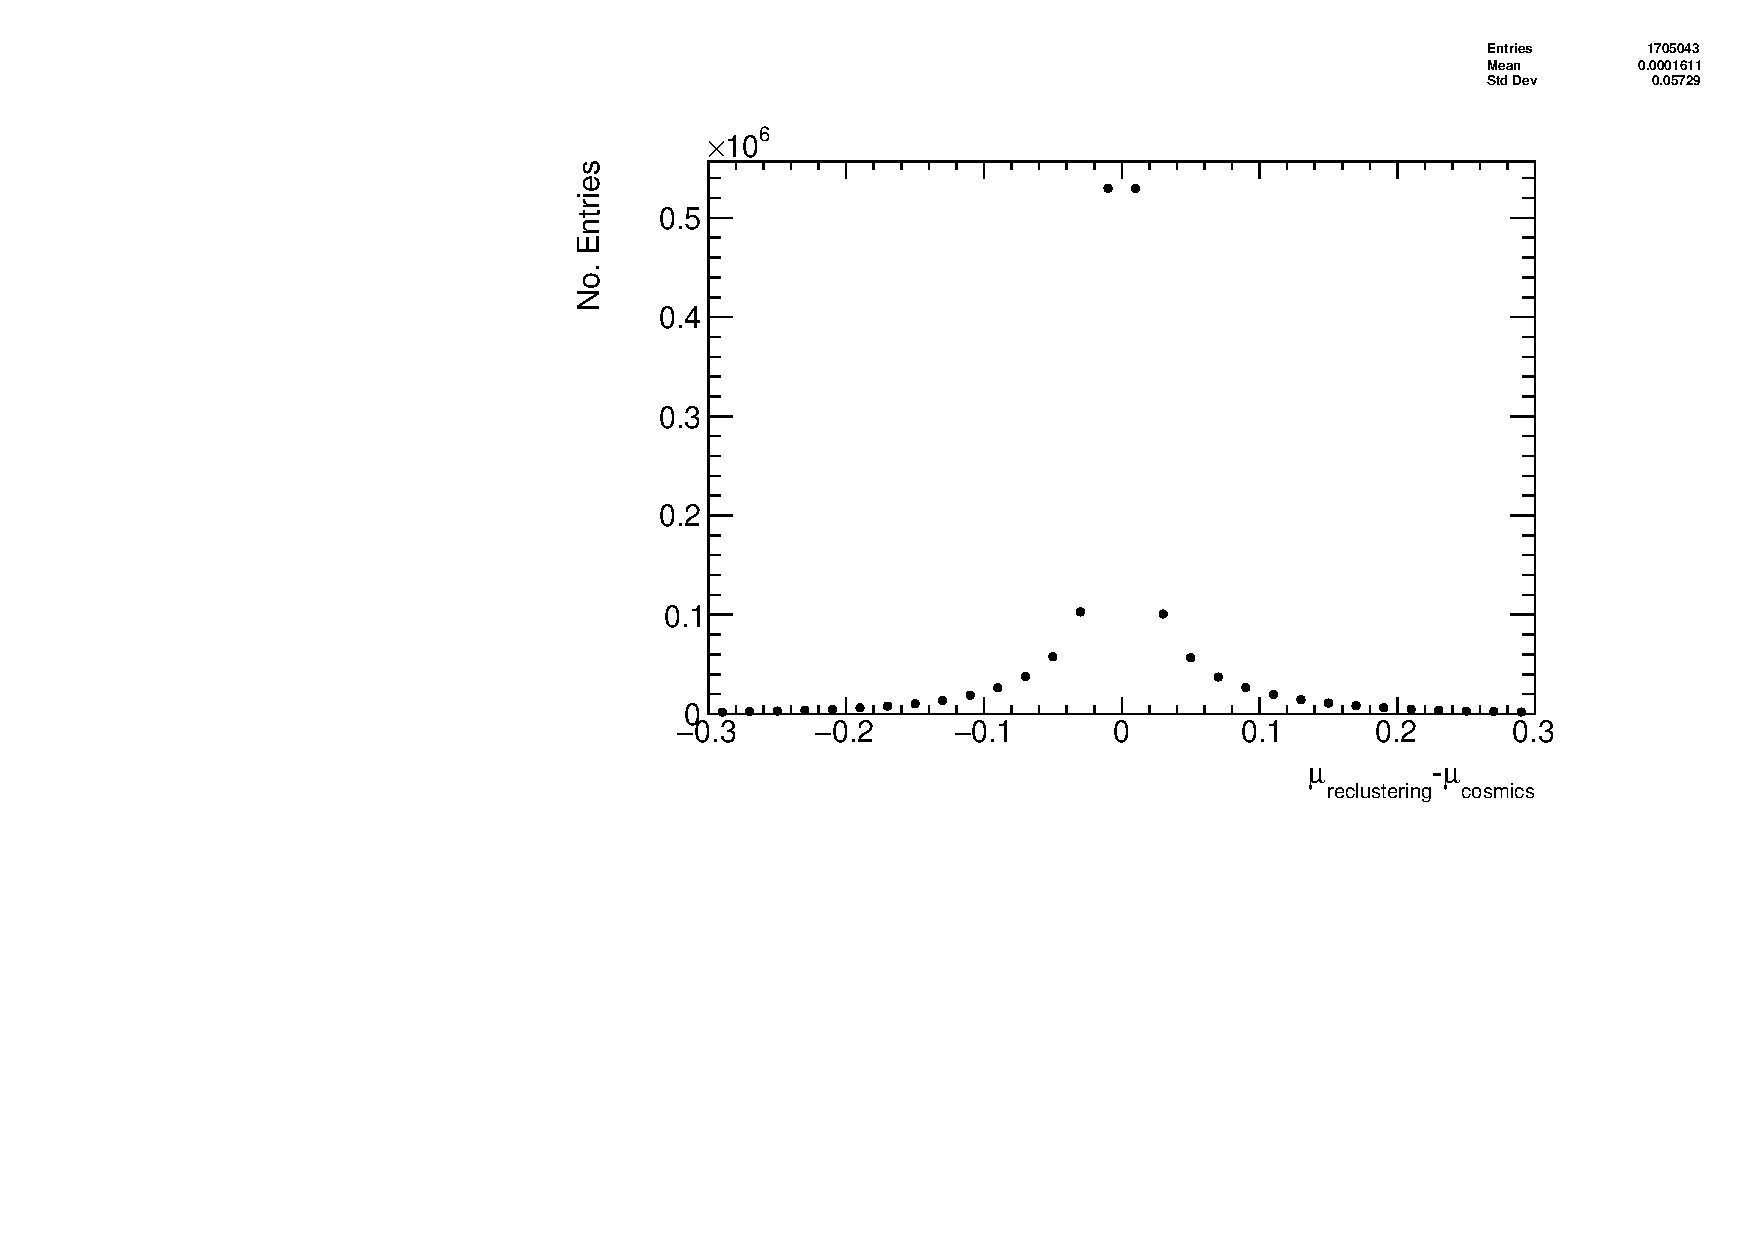
\includegraphics[width = \textwidth]{figures/figure_QL2P08_3100V_2021-05-21_reclustering_plots_mu_reclustering_minus_mu_cosmics.pdf}
    \caption{The difference between cluster means calculated with Guo's method~\cite{guo_simple_2011} and Minuit2 for ROOT~\cite{hatlo_developments_2005} for data collected with QL2.P.8 at \SI{3.1}{kV}.}
    \label{fig:mu_reclustering_minus_mu_cosmics}
\end{figure}

The difference in cluster means calculated with each algorithm is centered around zero indicating that the two algorithms are not biased with respect to one another. The RMS of the distribution in Figure~\ref{fig:mu_reclustering_minus_mu_cosmics} is \SI{57}{\micro\meter}, which is much larger than the statistical uncertainty in the mean calculated by the Minuit2 algorithm, which peaks around \SI{7}{\micro\meter}. There is no reason to suspect that one algorithm calculates a more accurate mean that the other, so the uncertainty in the cluster mean should account for the variation between algorithms. An RMS of ~\SI{60}{\micro\meter} was common for data taken with a sample of quadruplets at \SI{3.1}{kV}. Therefore, a conservative estimate of the uncertainty in the reconstructed cluster $y$-coordinate is \SI{60}{\micro\meter}.

% --------------------------------------------------
% \section{Effect of uncertainty in cluster mean on track residuals}
% --------------------------------------------------

%\label{sec:appendix_clustering_track_residuals}
%The uncertainty assigned to the hit position affected the uncertainty in the extrapolated/interpolated position of the track, and in the residuals. The bin size of the residual distributions was set to \SI{200}{\micro\meter} because that was the uncertainty in the residuals calculated from the tracks with the least favourable geometry (like tracks built from hits on layers 1 and 2 and extrapolated to layer 4). 
